\subsection {Inteligencia artificial}\label{subsec:intela}
\begin{wrapfigure}{r}{5.6cm}
	\begin{tikzpicture}
	\def\IA{(0,0) circle (2.8cm)}
	\def\AM{(270:1.4cm) circle (1.4cm)}
	\def\AP{(270:2.1cm) circle (.7cm)}
	\draw \IA node[above]{$\overset{\text{Inteligencia artificial}}{}$};
	\draw \AM node[above]{\tiny $\overunderset{\text{Aprendizaje}}{\text{maquinal}}{}$};
	\draw \AP node{\tiny $\overunderset{\text{Aprendizaje}}{\text{profundo}}{}$};
	\end{tikzpicture}\centering\\
{\scriptsize El aprendizaje profundo es un sub}
\end{wrapfigure}\cite{cho18}\label{fig:AI}
\emph{Inteligencia artificial} es definida como ``el esfuerzo por automatizar tareas intelectuales normalmente realizadas por humanos''\cite{cho18}, de este campo general se desprenden el \emph{aprendizaje maquinal} y el \emph{aprendizaje profundo}.



%\begin{figure}[H]\centering
%\begin{tikzpicture}
%\def\IA{(0,0) circle (1.5cm)}
%\def\AM{(270:.7cm) circle (.75cm)}
%\def\AP{(270:1.025cm) circle (.375cm)}
%\draw \IA node[above]{IA};
%\draw \AM node[above]{AM};
%\draw \AP node{AP};
%\end{tikzpicture}
%\caption{Aprendizaje profundo (AP), es un subcampo del aprendizaje maquinal (AM), que a su vez es un subcampo de la inteligencia artificial (IA)\cite{cho18}.}\label{fig:AI}
%\end{figure}
\subsubsection {Aprendizaje maquinal}\label{subsec:machinel}
La definición de aprendizaje maquinal de Tom Mitchell\cite{mich19} dice que ``un programa de computadora aprende de experiencia $E$ con respecto a una tarea $T$ y una medición de rendimiento $P$, si su rendimiento en $T$, medido por $P$, mejora con experiencia $E$.''

Esto dignifica que a diferencia del paradigma clásico de programación, donde los humanos introducen órdenes y datos para ser procesados de acuerdo con dichas reglas, en el aprendizaje maquinal el humano introduce datos y respuestas esperadas de estos datos obteniendo como resultado las reglas, es decir, si no es programado explícitamente, entonces un sistema de aprendizaje maquinal es entrenado: se le presentan muchos ejemplos relevantes a una tarea, y si encuentra una estructura estadística en ellos, genera reglas para automatizar la tarea.
\subsubsection {Procesamiento de lenguaje natural}\label{subsec:nlp}
\#\#\#\#\#\#\#\#\#\#\#\#\#\#\#\#\#\#\#\#\#\#\#\#\#\#\#\#\#\#\#\#\#\#\#\#\#\#\#\#\#\\
tengo que cambiar cómo estoy ML y NLP, parece que son lo mismo (porque uno viene o complementa al otro actualmente), resumir ambos en ML y agregar info de morfemas y todo ese rollo

\#\#\#\#\#\#\#\#\#\#\#\#\#\#\#\#\#\#\#\#\#\#\#\#\#\#\#\#\#\#\#\#\#\#\#\#\#\#\#\#\#\\
El \emph{procesamiento de lenguaje natural}, es el conjunto de métodos para hacer accesible el lenguaje humano a las computadoras\cite{eise19}. Existen dos enfoques en lo que debe ser su tarea central: 
\begin{itemize}
	\item Entrenar sistemas de principio a fin para que transmuten texto sin procesar en cualquier estructura deseada.
	\item Transformar texto en una pila de estructuras lingüísticas de uso general que en teoría deben poder soportar cualquier aplicación.
\end{itemize}
Dos de los módulos básicos de NLP son \emph{búsqueda} y \emph{aprendizaje} con los que se puede resolver muchos problemas que podemos describir en la siguiente forma matemática
\begin{equation}
\begin{matrix}
\hat{y}=argmax\Psi(x,y;0),\\
y\in Y(x)
\end{matrix}
\end{equation}
donde,
\begin{itemize}
	\item $x$ es la entrada, un elemento de un conjunto $X$.
	\item $y$ es el resultado, un elemento de un conjunto $Y$.
	\item $\Psi$ es una función de puntuación (también conocida como \emph{modelo}), que va desde el conjunto $X\times Y$ hasta los números reales.
	\item $\emptyset$ es el vector de parámetros para $\Psi$.
	\item $\hat{y}$ es el resultado previsto, que es elegido para maximizar la función de puntuación.
\end{itemize}
El módulo de búsqueda se encarga de computar el $argmax$ de la función $\Psi$, es decir, encuentra el resultado $\hat{y}$ con la mejor puntuación con respecto a la entrada $x$. El módulo de aprendizaje encuentra los parámetros $\theta$ por medio del procesamiento de grandes conjuntos de datos de ejemplos etiquetados ${\{(x^i,y^i)\}}_{i=1}^{N}$.